%%%% MEASURING TREASURY DEBT AND MARKET DEPTH %%%%
%%%%%%%%%%%% CONFERENCE PRESENTATION %%%%%%%%%%%%%


%:PREAMBLE

% << Handout Slide Version >> %
\documentclass[11pt, handout, aspectratio=169]{beamer}

% << Class Slide Version >> % 
%\documentclass[11pt, aspectratio=169]{beamer}


%:	THEMES
\usetheme{Madrid}
\usecolortheme{default}

%:	DEFINING COLORS
\definecolor{WeberPurple}{rgb}{.286, .137, .396}
\definecolor{WeberGray}{rgb}{.294, .286, .271}
\definecolor{WeberSecondary}{rgb}{.639, .569, .694}
\definecolor{blue}{RGB}{3, 59, 150}%{0,114,178}
\definecolor{red}{RGB}{213,94,0}
\definecolor{yellow}{RGB}{240,228,66}
\definecolor{green}{RGB}{0,158,115}
\definecolor{greyblue}{RGB}{178, 204, 247}
\definecolor{quizred}{RGB}{242, 52, 48}

%:	RESETTING TEMPLATE COLORS 
\setbeamercolor*{palette primary}{use=structure,fg=white,bg=WeberPurple}
\setbeamercolor*{palette secondary}{use=structure,fg=white,bg=WeberSecondary}
\setbeamercolor*{palette tertiary}{use=structure,fg=white,bg=WeberGray}
\setbeamercolor{local structure}{fg=WeberPurple}
\setbeamercolor{section in toc}{fg=WeberPurple}
\setbeamercolor{subsection in toc}{fg=WeberGray}
\setbeamercolor{block title}{bg=WeberPurple,fg=white}
\setbeamercolor{block body}{bg=WeberSecondary,fg=black}

%:	PACKAGES
\usepackage{amsmath}
\usepackage{amsthm}
\usepackage{amssymb}
\usepackage[retainorgcmds]{IEEEtrantools}
\usepackage{graphicx}
\usepackage{multicol}
\usepackage{multirow}
\usepackage[english]{babel}
\usepackage{color} 
\usepackage[labelformat=empty]{caption}
\usepackage{threeparttable}
\usepackage{dcolumn}
\newcolumntype{d}{D{.}{.}{3.4}}
\newcolumntype{v}{D{.}{.}{3.2}}
\newcolumntype{R}{>{\raggedleft\arraybackslash}X}
\usepackage{subfigure}
%\usepackage{appendixnumberbeamer}
\usepackage{epsfig}
\setbeamertemplate{bibliography item}{$\cdot$}
\usepackage{xfrac}
\usepackage[all]{xy}
\usepackage{tikz}
\usetikzlibrary{calc,intersections,positioning,patterns,decorations.pathreplacing}
\usepackage{wasysym}
\usepackage{tabularx}
\usepackage{booktabs}
\usepackage{eurosym}
\usepackage{framed} 	% For the career inserts
%\usepackage{epstopdf}
%\beamertemplatenavigationsymbolsempty
\usepackage{appendixnumberbeamer}

%:	ADJUSTING THE TABLE OF CONTENTS
\mode<presentation>{\AtBeginSection[]{
	\begin{frame}
    \frametitle{Roadmap of Today's Lecture}
    \tableofcontents[currentsection]
	\end{frame}
	}
	}
\makeatother

\mode<presentation>{
	\setcounter{tocdepth}{2}
}

%:	ADJUSTING ITMEIZE/ENUMERATE ENVIRONMENTS
\newenvironment{wideitemize}{\itemize\addtolength{\itemsep}{10pt}}{\enditemize} 
\newenvironment{wideenumerate}{\enumerate\addtolength{\itemsep}{10pt}}{\endenumerate}

%:	ADDING NEW ENVIRONMENTS
\newcolumntype{d}[1]{D{.}{.}{#1}}

\newcommand\mathcomment[2]{
	\tikz[baseline]{\node[anchor=base,inner sep=0pt,outer sep=2pt] (myterm) {$#1$};
	\node[overlay,anchor=south,yshift=1em] (mycomment) at (myterm.north) {#2};
	\draw[overlay,->] (mycomment.south) -- (myterm.north);
	}
}
\newcommand\mathcommentbelow[2]{
	\tikz[baseline]{\node[anchor=base,inner sep=0pt,outer sep=2pt] (myterm) {$#1$};
	\node[overlay,anchor=north,yshift=-1em, text width=3cm,align=center] (mycomment) at (myterm.south) {#2};
	\draw[overlay,->] (mycomment.north) -- (myterm.south);
}
}

%:TITLE MATERIAL
\title[Measuring Treasury Debt and Depth]{Measuring Treasury Debt and Market Depth}
\author[Keinsley]{Dr. Andrew Keinsley}
\institute[WSU]{Weber State University}
\date{November, 2023}

%:BEGIN DOCUMENT
\begin{document}

\frame{\maketitle}

%:	INTRODUCTION

\begin{frame}
\frametitle{The Basics}
\begin{columns}[t]
	\begin{column}{0.49\textwidth}
		\begin{wideitemize}
			\item US fiscal debt has come back into sharp focus recently
			\begin{itemize}
				\item COVID-19
				\item Industrial policy
				\item Inflation
				\item Rising interest rates
			\end{itemize}
			\item Traditional view of the UST market focuses on size, not depth 
		\end{wideitemize}	
	\end{column}
	\hfill
	\begin{column}{0.49\textwidth}
		\begin{wideitemize}
			\item {\bf \color{WeberPurple}{Contributions}}
			\begin{wideenumerate}
				\item Simple sum of USTs is incorrect
				\item Derivation of user cost of USTs
				\item Creation of index to track true aggregate
				\item Value of USTs directly impacts fiscal sustainability
			\end{wideenumerate}
		\end{wideitemize}
	\end{column}
\end{columns}
\end{frame}

%:	QUALITIES OF THE UST MARKET

\begin{frame}
	\label{slide:UST_Market}
	\frametitle{USTs are Imperfect Substitutes}
	\vspace{-2em}
	\begin{columns}[t]
		\begin{column}{0.49\textwidth}
			\begin{center}
				\Large \textcolor{WeberPurple}{Literature}
			\end{center} \vspace{-.2in}
			{\color{WeberPurple}\rule{\linewidth}{2pt}}
			\begin{wideitemize}
				\item Krishnamurthy and Vissing-Jorgensen (2012, 2013)
				\item Nagel (2016) \\ $\vdots$
				\item All: the various maturities/types of UTSs have different attributes/purposes
			\end{wideitemize}
		\end{column}
		\hfill
		\begin{column}{0.49\textwidth}
			\begin{center}
				\Large \textcolor{WeberPurple}{Findings}
			\end{center} \vspace{-.2in}
			{\color{WeberPurple}\rule{\linewidth}{2pt}}
			\begin{wideitemize}
				\item Extension of Amihud and Mendelson (1991)
				\begin{itemize}
					\item Match securities that mature within one day of each other
					\item Regress YTM spreads against a variety of factors
				\end{itemize}
				\item {\bf \color{WeberPurple}{Contribution}}
				\begin{itemize}
					\item Bills are a liquidity hedge
					\item Bonds are a savings vehicle
					\item They should not be linearly aggregated 
				\end{itemize}
			\end{wideitemize}
		\end{column}
	\end{columns}
	\vfill
	\hfill \hyperlink{slide:Model}{\beamerbutton{Details}}
\end{frame}

\begin{frame}
\frametitle{The User Cost of Treasury Securities}
\label{slide:UserCost}
\begin{columns}[t]
	\begin{column}{0.49\textwidth}
		\begin{wideitemize}
			\item A proper index number
			\begin{itemize}
				\item Not the aggregate, itself
				\item Tracks the aggregate nonparmetrically
				\item Must be derived from optimization 
			\end{itemize}
			\item Standard single-period user cost
				$$\eta_t = \frac{R_t-r_t}{1+R_t}$$
			\begin{itemize}
				\item Barnett (1978)
				\item Opportunity cost of holding the asset
			\end{itemize}
		\end{wideitemize}	
	\end{column}
	\hfill
	\begin{column}{0.49\textwidth}
		\begin{wideitemize}
			\item Partial equilibrium model: household
			\begin{itemize}
				\item Standard utility maximization
				\item Short- and long-term bonds, and a benchmark asset
			\end{itemize}
			\item {\bf \color{WeberPurple}{Contribution}}
			\begin{itemize}
				\item Deriving the single-period user cost of a long-term asset
			\end{itemize}
		\end{wideitemize}
	\end{column}
\end{columns}
	\vfill
	\hfill \hyperlink{slide:Utility}{\beamerbutton{Details}}
\end{frame}

\begin{frame}
\frametitle{The User Cost of Long-Term Treasury Securities}
\begin{equation*}
	\eta^L_t = \frac{\mathbb{E}_t \Big[ \frac{\mu_{t+1}}{\mu_{t}}\frac{1}{\pi_{t+1}} \Big\{ \mathcomment{\color{blue}{R^n_t  - (1-\delta)\gamma_{3,t+1}\Delta R^n_{t+1}}}{\it one-period return, benchmark} - \mathcomment{\color{red}{\left(r^{L,n}_t - (1-\alpha)\gamma_{4,t+1}\Delta r^{L,n}_{t+1}\right)}}{\it long-term bond}\Big\}\Big]}{\mathbb{E}_t \Big[ \frac{\mu_{t+1}}{\mu_{t}}\frac{1}{\pi_{t+1}} \Big\{ 1+ {\color{blue}{R^n_t - (1-\delta)\gamma_{3,t+1}\Delta R^n_{t+1}}}\Big\}\Big]}
\label{eq:usercost_LT}
\end{equation*}
\vfill
\begin{wideitemize}
	\item $R^n_t, r^{L,n}_t$ are ``coupon" rates \tikz[remember picture] \coordinate (A);
	\item $\gamma_{i,t+1}$ is the expected price \tikz[remember picture] \coordinate (B);
	\item $\delta, \alpha \in (0,1]$ are the maturity rates
	% \begin{itemize}
	% 	\item $\delta, \alpha = 1$ reduces to the standard user cost
	% \end{itemize}
\end{wideitemize}
\begin{tikzpicture}[overlay, remember picture]
	\draw[thick,decorate,decoration={brace,amplitude=5pt, segment length=1cm, aspect=0.5}] 
		([xshift=1em]A.east) -- ([xshift=1.2em]B.east) 
		node[midway,right,xshift=0.5cm] {$\gamma_{3,t+1}\Delta R^{n}_{t+1}$ is the expected capital gain};
\end{tikzpicture}
\end{frame}


\begin{frame}
\frametitle{Data and Baseline Result}
\label{slide:BaselineResult}
\begin{columns}[t]
	\begin{column}{0.45\textwidth}
		\begin{wideitemize}
			\item Center for Research in Securities Pricing (CRSP)
			\item CUSIP-level, monthly data on US Treasuries: 1977-2020
			\item 1-month ahead forward rates used for expected values
			\item Fisher-ideal index functional form 
			\begin{itemize}
				\item Securities separated by type
				\item Then separated by quarters to maturity
			\end{itemize}
		\end{wideitemize}	
		\hfill \hyperlink{slide:InitialResult}{\beamerbutton{Initial Results}}
	\end{column}
	\hfill
	\begin{column}{0.55\textwidth}
		\begin{figure}[h]
			\centering
			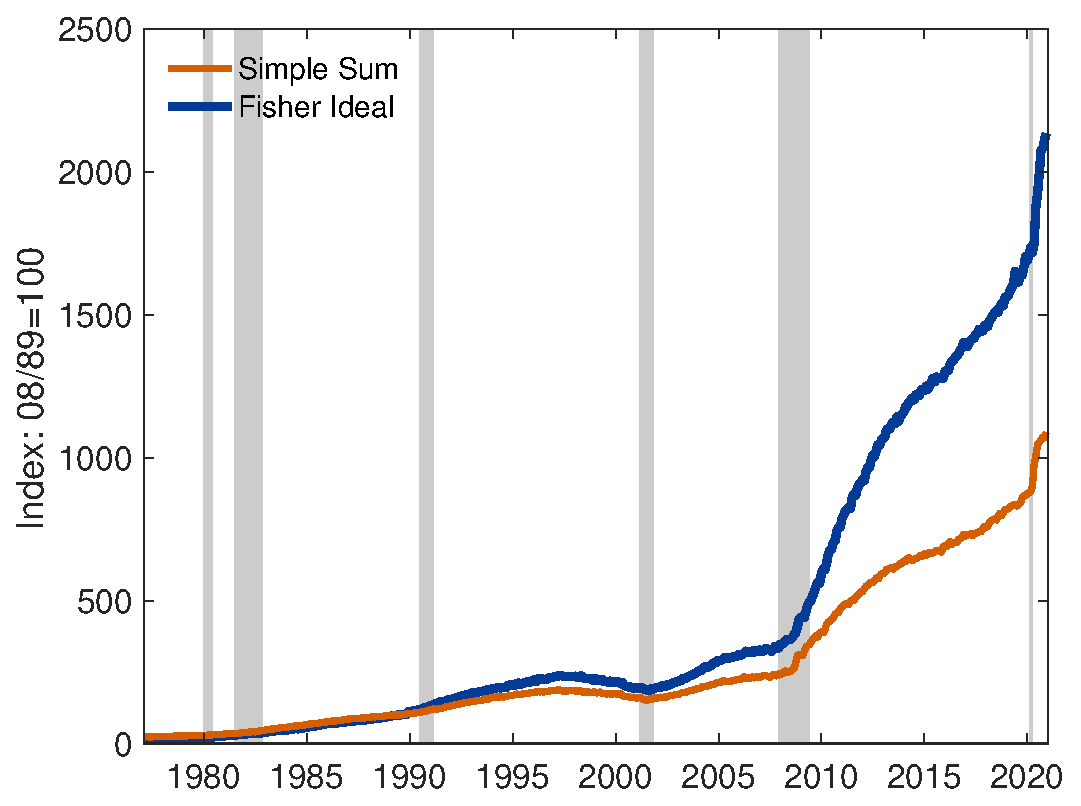
\includegraphics[width=\textwidth]{../Figures/FisherIndex_v2.eps}
			% \caption{Aggregate}
			% \label{fig:MS_Index}
		\end{figure}
	\end{column}
\end{columns}
\end{frame}

\begin{frame}
\frametitle{Extracting the Monetary Services of Treasury Securities}
\begin{columns}[t]
	\begin{column}{.45\textwidth}
		\vspace{2em}
		\begin{equation*}
			% \mathcomment{
				{\color{blue}\%\Delta(\text{Quantity}+\text{Monetary Services})}
				% }{\it Fisher Ideal Index}
		\end{equation*} \vfill
		\begin{equation*}
			-
			% \mathcomment{
				{\color{red}\%\Delta(\text{Quantity})}
				% }{\it Simple Sum}
		\end{equation*} \vfill
		\begin{equation*}
			= \%\Delta(\text{Monetary Services})
		\end{equation*}
	\end{column}
	\begin{column}{.55\textwidth}
		\begin{figure}[p]
			\centering
			\includegraphics[width=\textwidth]{../Figures/MonetaryServices_Index.eps}
			% \caption{Derived Monetary Services Quantity Index}
			% \label{fig:MS_Index}
		\end{figure}
	\end{column}
\end{columns}
\end{frame}

\begin{frame}
\frametitle{It's all Relative}
\begin{columns}[t]
	\begin{column}{.45\textwidth}
		\begin{wideitemize}
			\item This index is a measure of the ``depth" of the market
			\item More recent movements align with
			\begin{itemize}
				\item Budget surpluses of the 1990s
				\item European debt crisis of the 2010s
				\item COVID-19 ``dash for cash''
			\end{itemize}
		\end{wideitemize}
	\end{column}
	\begin{column}{.55\textwidth}
		\begin{figure}[p]
			\centering
			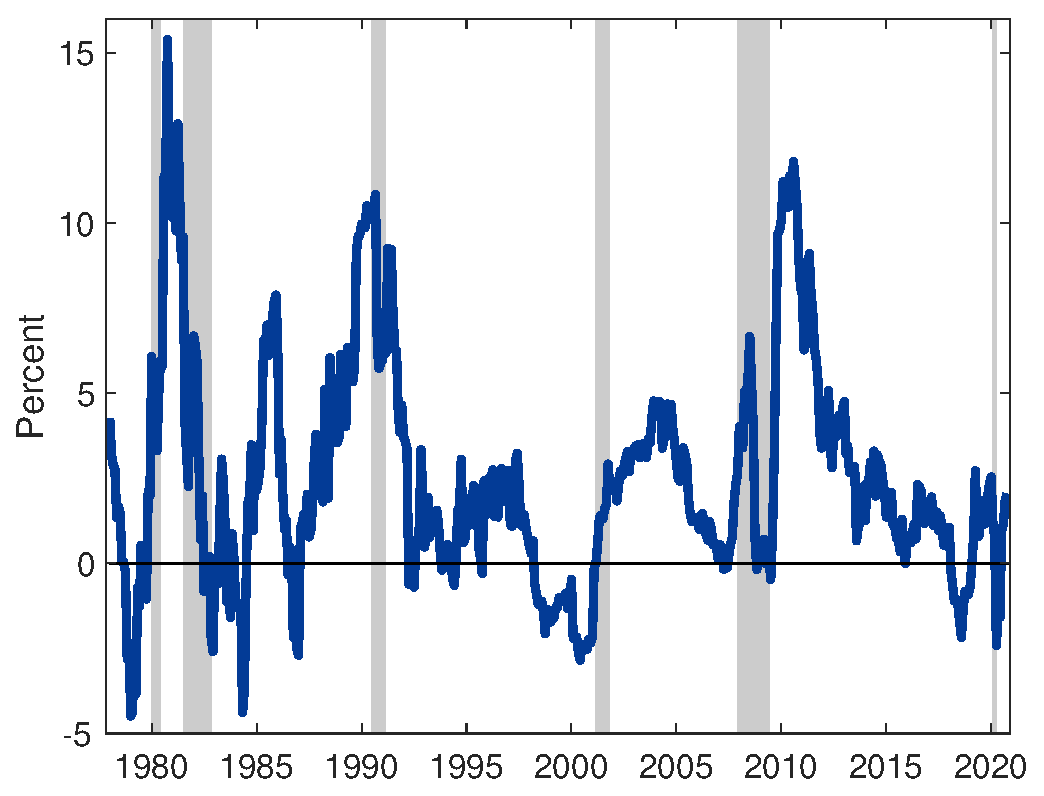
\includegraphics[width=\textwidth]{../Figures/YoYGrowth_MonServices.eps}
			% \caption{Year-over-year Growth of Fiscally-Supplied Monetary Services}
			% \label{fig:YoY_Growth}
		\end{figure}
	\end{column}
\end{columns}
\end{frame}

\begin{frame}
\frametitle{The Value of Treasury Securities}
\begin{columns}[t]
	\begin{column}{.45\textwidth}
		\begin{wideitemize}
			\item Traditional accounting of fiscal capacity relies on the simple sum of USTs
			\item The analysis here shows that this is incorrect
			\item USTs provide a monetary service to the economy
		\end{wideitemize}
	\end{column}
	\begin{column}{.55\textwidth}
		\begin{wideitemize}
			\item Brunnermeier, Merkel and Sannikov (2022)-like analysis
			\item {\bf \color{WeberPurple}{Contribution}}
			\begin{itemize}
				\item The value of USTs directly contributes to fiscal sustainability
				\item Also see the tradeoffs faced when considering a portfolio of USTs with varying maturities
			\end{itemize}
		\end{wideitemize}
	\end{column}
\end{columns}
\end{frame}

\begin{frame}
\frametitle{Fiscal Capacity and the Value of USTs}
\begin{multline*}
	\frac{B_{t-1} + B^L_{t-1}}{p_t}(1+r_{t-1})= \mathcomment{\color{blue}{s_t}}{\color{blue}{Primary surplus}}  - \mathcomment{\color{red}{(r_{t-1}^L - r_{t-1})\frac{B^L_{t-1}}{p_t}}}{\color{red}{Spread Component}} + \beta\mathbb{E}_t\left[\frac{\mu_{1,t+1}}{\mu_{1,t}} \frac{B_{t} +B^L_{t}}{p_{t+1}}(1+r_{t})\right] \\ 
		+ \mathcommentbelow{\color{brown}{\beta\mathbb{E}_t\left[\frac{\mu_{1,t+1}}{\mu_{1,t}} \frac{B^L_{t}}{p_{t+1}}(1+r^L_{t} - (1-\alpha)\gamma_{4,t+1}\Delta r^{L,n}_{t+1} - r_t)\right]}}{\color{brown}{Relative Holding-Period Return}} 
		+  \mathcommentbelow{\color{WeberPurple}{\gamma_{2,t}\frac{M_t}{p_t}}}{\color{WeberPurple}{Value of Monetary Services}}
	\label{eq:fiscalcapacity}
\end{multline*}
\vfill
\begin{wideitemize}
	\item $M_t$ is stock of monetary services
	\item $\gamma_{2,t}$ is the price dual of those monetary services
	\item Thus, the value of these monetary services directly adds to fiscal capacity
\end{wideitemize}
\end{frame}

\begin{frame}
\frametitle{The Value of these Monetary Services}
\begin{columns}
	\begin{column}{.45\textwidth}
		\begin{wideitemize}
			\item Price dual via Fisher's factor reversal
			\item Further exploration of this is needed
			\begin{itemize}
				\item Fiscal sustainability
				\item Inflation
				\item Monetary policy
			\end{itemize}
		\end{wideitemize}
	\end{column}
	\begin{column}{.55\textwidth}
		\begin{figure}[p]
			\centering
			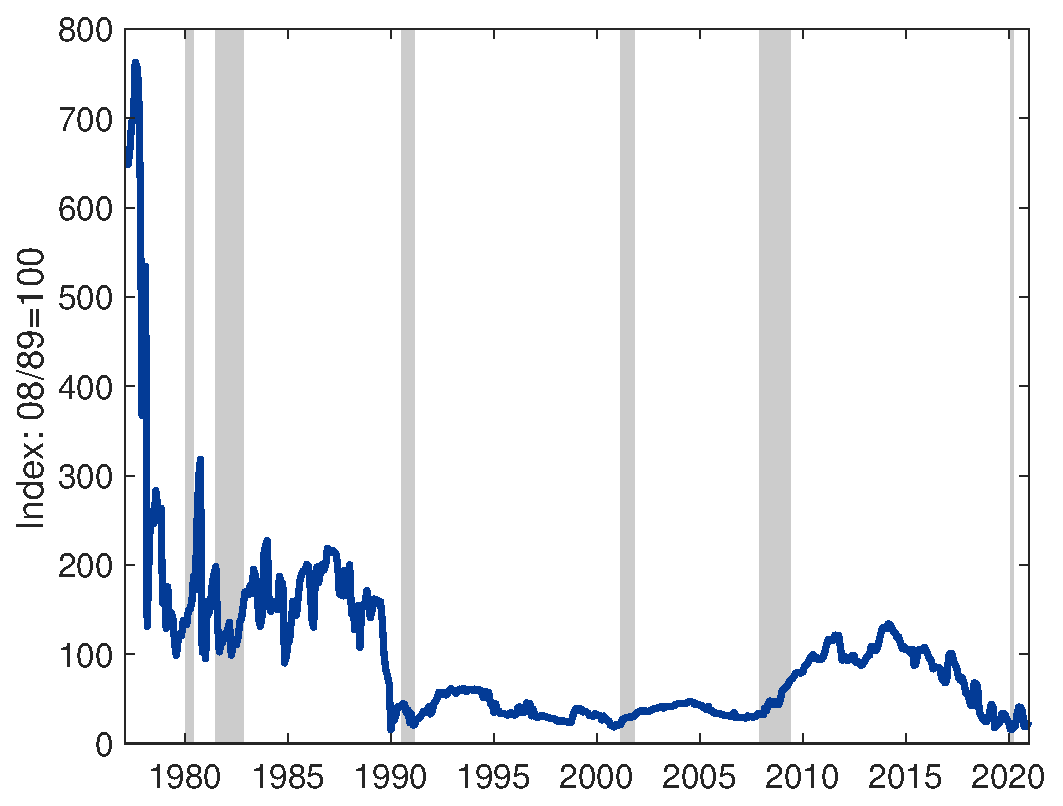
\includegraphics[width=\textwidth]{../Figures/FiscalCapacity_Index.eps}
			% \caption{Value of Fiscal Monetary Services}
			% \label{fig:FiscalServices_Value}
		\end{figure}
	\end{column}
\end{columns}
\end{frame}

\begin{frame}
\frametitle{Conclusion}
\begin{columns}[t]
	\begin{column}{.45\textwidth}
		\begin{wideitemize}
			\item {\bf \color{WeberPurple}{Contributions}}
			\begin{enumerate}
				\item Simple sum of USTs is incorrect
				\item Derivation of user cost of USTs
				\item Creation of index to track true aggregate
				\item Value of USTs directly impacts fiscal sustainability
			\end{enumerate}
			\item USTs are more than just the sum of their principal value
		\end{wideitemize}
	\end{column}
	\begin{column}{.55\textwidth}
		\begin{wideitemize}
			\item {\bf \color{WeberPurple}{Extensions}}
			\begin{itemize}
				\item Applications to sovereign debt crises
				\item Expansion of the measure to include risk
				\item Refining the basket of securities
				\item Monetary-Fiscal interaction and inflation
			\end{itemize}
		\end{wideitemize}
	\end{column}
\end{columns}
\end{frame}

\begin{frame}
	\frametitle{Thank You!}
	\begin{center}
		\LARGE \textcolor{WeberPurple}{Questions?}
	\end{center}
\end{frame}

%:	APPENDIX
\appendix
\setcounter{framenumber}{0}

\begin{frame}
	\begin{center}
		\LARGE \textcolor{WeberPurple}{\it Appendix Slides}
	\end{center}
\end{frame}
	
\begin{frame}
	\frametitle{Bond Market Segmentation: Model}
	\label{slide:Model}
	\begin{columns}[t]
		\begin{column}{0.49\textwidth}
			\begin{wideitemize}
				\item Data
				\begin{itemize}
					\item USTs: separated by nominal type
					\item Oct 1996--Dec 2020 subsample
				\end{itemize}
				\item Methodology
				\begin{itemize}
					\item Matching by days to maturity
					\item Bill matches: 6 months maturity or less
					\item Dependent variable: YTM spread
					$$\text{spread: } \text{``senior''}-\text{``junior''} $$
				\end{itemize}
			\end{wideitemize}
		\end{column}
		\begin{column}{0.49\textwidth}
			\begin{wideitemize}
				\item Independent Variables
				\begin{enumerate}
					\item Relative bid-ask spread
						$$ \frac{\text{ask price }-\text{ bid price}}{\text{ask price }+\text{ accrued interest}}\times 100.$$
					\item Coupon rate spread
					\item Months/years to maturity
					\item 10y-2y spread
					\item Constant
				\end{enumerate}
			\end{wideitemize}
		\end{column}
	\end{columns}
	\vfill
	\hfill \hyperlink{slide:UST_Market}{\beamerbutton{Back}}
\end{frame}

\begin{frame}
	% \frametitle{Empirical Results}
	\begin{table}[p]
		\centering
		\setlength{\tabcolsep}{15pt}
		\renewcommand{\arraystretch}{1.2}
		% \caption{Relative Liquidity and Yield to Maturity$^a$} \vspace{1em}
		\label{tab:Relative_Liquidity}
		\resizebox{\textwidth}{!}{
		\begin{threeparttable}
			\begin{tabular}{l d{2.4} d{2.4} d{2.4}} \toprule
											& \multicolumn{1}{c}{Notes--Bills}  	& \multicolumn{1}{c}{Bonds--Notes} 	& \multicolumn{1}{c}{Bonds--Bills}	\\ \midrule
				Relative Bid-Ask Spread 	& 0.4163^{**}								& 0.0981							& -0.1424^{**}		 					\\ [-0.5em]
											& (0.173)									& (0.074)							& (0.074)	 						\\
				Coupon Rate Spread 			& 0.0210^{***}								& 0.0170^{***}						& 0.0076 							\\ [-0.5em]
											& (0.001)									& (0.005)							& (0.013)	 						\\
				% Months to Maturity 			& -0.0152^{***} 							& 									& -0.1028^{***}								 	\\ [-0.5em]
				% 							& (0.002)									&									& (0.018)									\\
				% Years to Maturity 			& 											& -0.0049^{***}						& 			 					\\ [-0.5em]
				% 							& 											& (0.001)							& 		 						\\
				% Year Dummy 					& 0.0027^{***}								& -0.0079^{***}						& -0.0079 			\\ [-0.5em]
				% 							& (0.001) 									& (0.001)							& (0.001)	 		\\ 
				10y-2y Spread 				& 0.0234^{***}								& -0.0124^{***}						& -0.0484 					\\ [-0.5em]
											& (0.003) 									& (0.002)							& (0.033)	 						\\ 
				\vdots						& \vdots 									& \vdots 							& \vdots 							\\\midrule
				% Constant					& 0.0076 									& -0.0554^{**}						& -0.3244^{**} 						\\ [-0.5em]
				% 							& (0.010)									& (0.030) 							& (0.154)  							\\\midrule
				Observations				& \multicolumn{1}{c}{2250}					& \multicolumn{1}{c}{7430}			& \multicolumn{1}{c}{78} 			\\
				R-Squared					& 0.207										& 0.505								& 0.399			 					\\
				F-statistic 				& 99.48										& 207.2								& 20.19			 					\\ \bottomrule 
			\end{tabular}
			% \begin{tablenotes}
			% 	\item[a] \footnotesize{The dependent variable is the yield-to-maturity spread between securities matched by thier respective days to maturity. Standard errors are heteroskedasticity robust (HC1). Designations ***, **, and * represent results that are statistivally significant at the one, five, and ten percent levels, respecitivly.}
			% 	\item[b] \footnotesize{Analyses considering Treasury bills are limited to those securities with six months to maturity or less. This ensures that both securities have no other payments remaining until the maturity date.}
			% \end{tablenotes}
		\end{threeparttable}}
	\end{table}
	\vfill
	\hfill \hyperlink{slide:UST_Market}{\beamerbutton{Back}}
\end{frame}


\begin{frame}
\frametitle{Bonds in the Utility Function}
\label{slide:Utility}
\begin{columns}[t]
	\begin{column}{0.49\textwidth}
		\begin{wideitemize}
			\item Analysis of USTs is relative to USTs only
			\begin{itemize}
				\item Bonds are still liquid overall
				\item Bills are still safe overall
				\item Modeling this way avoids larger assumptions
			\end{itemize}
			\item Simple frictions to capture liquidity, etc.\ can be represented in a money-in-the-utility setting
			\item Use of $\text{MB} = \text{MC}$
			\begin{itemize}
				\item Left side: parametarized assumptions
				\item Right side: equivalent, nonparametric form
			\end{itemize}
		\end{wideitemize}
	\end{column}
	\begin{column}{0.49\textwidth}
		\begin{equation*}
			\max\mathbb{E}_t\! \sum^\infty_{t=0} \beta^t\left\{u(c_t) + v\left(m_t\right) + x(1-l_t)\right\}
			\label{eq:HH_Utility}
		\end{equation*}
		\begin{wideitemize}
			\item $m_t$: monetary services $\sim$ second-order translog function
			\begin{enumerate}
				\item an exact aggregator function
				\item second-order Taylor approximation of unknown aggregator
				\item second-order approximation to a CES function 
			\end{enumerate}
			\hfill (Boisvert, 1982)
		\end{wideitemize}
		\vfill
		\hfill \hyperlink{slide:UserCost}{\beamerbutton{Back}}
	\end{column}
\end{columns}
\end{frame}
	
\begin{frame}
\frametitle{Initial, Monthly Results}
\label{slide:InitialResult}
\begin{columns}[b]
	\begin{column}{0.95\textwidth}
		\begin{figure}
			\centering
			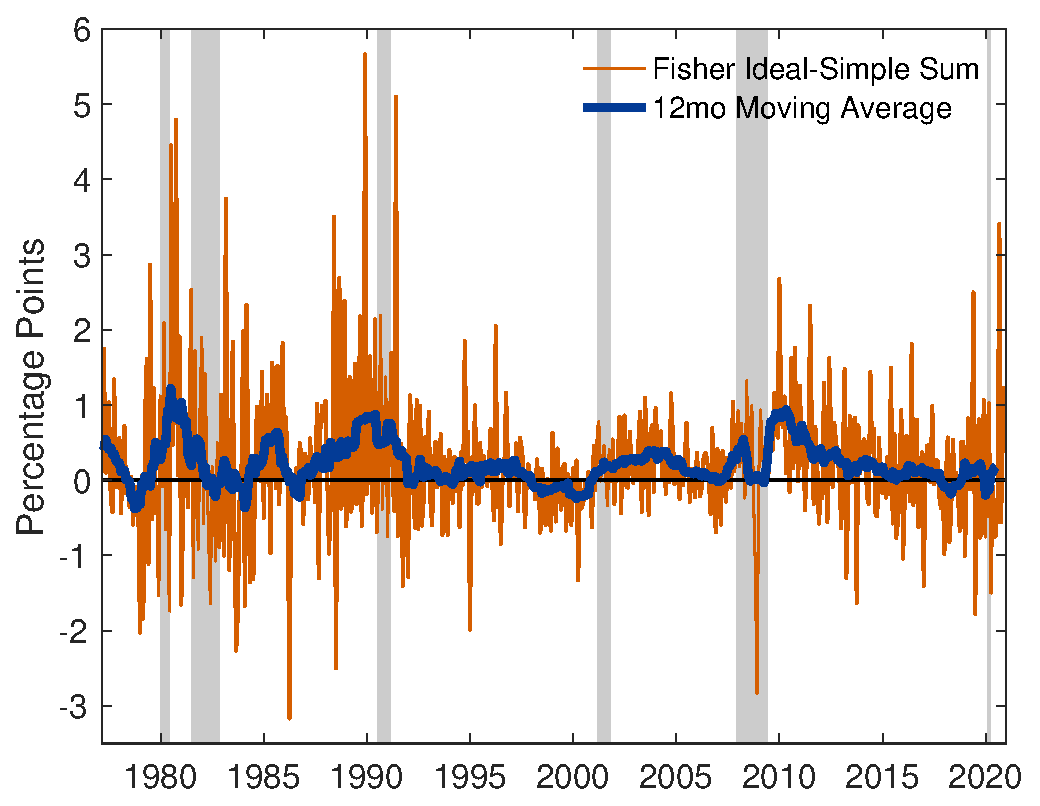
\includegraphics[width=0.63\textwidth]{../Figures/GrowthDiff_v2.eps}
		\end{figure}
	\end{column}
	\begin{column}{0.05\textwidth}
		\vfill
		\hfill \hyperlink{slide:BaselineResult}{\beamerbutton{Back}}
	\end{column}
\end{columns}
\end{frame}

\end{document}